\subsection{Contribution}
We introduce a passive controller that incorporates into the feedback control loop as visualized in Figure~\ref{fig:control_scheme_passive}. 
In this work, we make the following contributions:
\begin{itemize}
\item A novel obstacle-aware passive controller
(Sec.~\ref{sec:obstacle_aware_passivity})
\item A passivity guarantee (without storage tank) which applies to general damping controllers (Theorem~\ref{theorem:passivity})
\ifthesis
{}
\else
\item A collision avoidance analysis which provides insight into the path consistency around obstacles (Sec.~\ref{sec:collision_avoidance})
\fi
\iflong
\item Discrete-time analysis to enable control parameter design which ensures stability (Section~\ref{sec:discrete_time_behavior})
\else
% \editcolor{
% \item Discrete-time analysis to enable control parameter design which ensures stability (in extended artice \parencite{passive2024huber_extended})
% }
\fi
\item Implementation and testing on 7DoF robot arm (Sec.~\ref{sec:evaluation})
\end{itemize}

\begin{figure}[thb]
  \center
  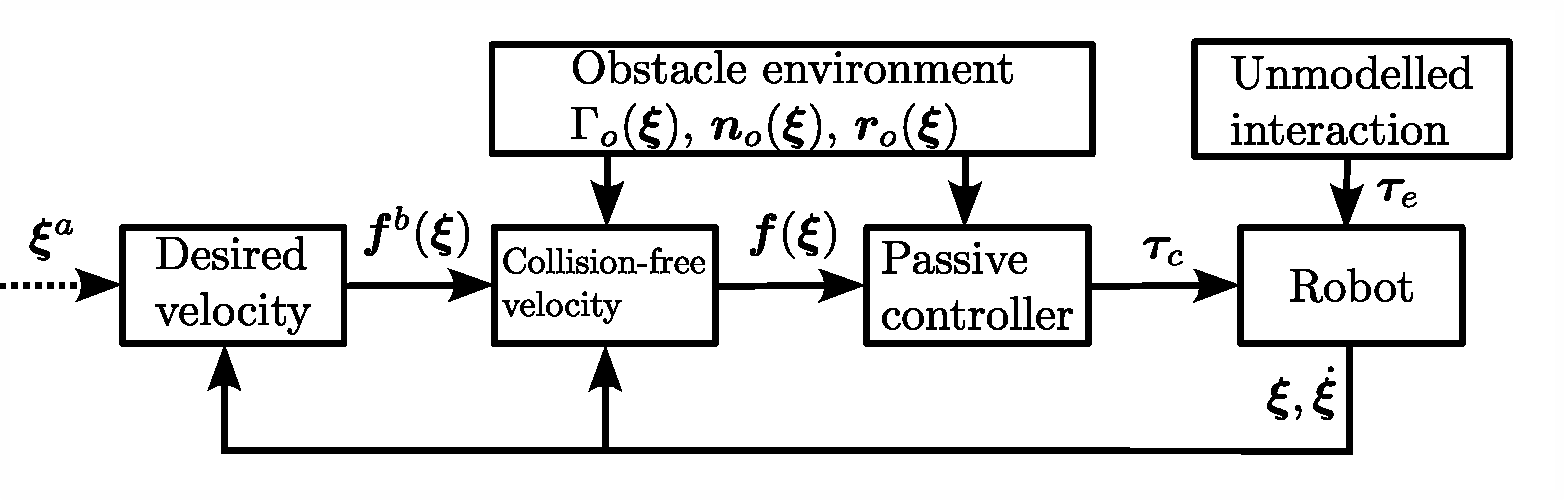
\includegraphics[width=1.0\columnwidth]{figures/control_scheme_passive.pdf}
\caption{The desired velocity $\vect f^b(\vecs \xi)$ can result from a learned velocity field or pointing towards a desired attractor $\vecs \xi^a$. The desired velocity is used to evaluate the obstacle avoidance velocity $\vect f(\vecs \xi)$, fed into the force controller to obtain the control force $\vect \tau_c$. In order to achieve collision avoidance, the distance function $\Gamma_o(\vecs \xi)$, the normal direction $\vect n_o(\vecs \xi)$, and the reference direction $\vect r_o(\vecs \xi)$ are evaluated for each obstacle $o = 1, ..., N^\mathrm{{obs}}$.}
\label{fig:control_scheme_passive}
\end{figure}
